\documentclass{beamer} 


% theme color
\definecolor{theme}{RGB}{28,90,127}
\definecolor{themelight}{RGB}{109,184,227}
\usecolortheme[named=theme]{structure} 

% outer color
%\usecolortheme{whale}
%\usecolortheme{seahorse}
\usecolortheme{dolphin}

% inner color
%\usecolortheme{lily}
\usecolortheme{orchid}
%\usecolortheme{rose}


% modified version of default frametitle with horizontal separation line
\makeatletter
\setbeamertemplate{frametitle}{
  \ifbeamercolorempty[bg]{frametitle}{}{\nointerlineskip}%
  \@tempdima=\textwidth%
  \advance\@tempdima by\beamer@leftmargin%
  \advance\@tempdima by\beamer@rightmargin%
  \begin{beamercolorbox}[sep=0.3cm,left,wd=\the\@tempdima]{frametitle}
    \usebeamerfont{frametitle}%
    \vbox{}\vskip-2ex%
    \if@tempswa\else\csname beamer@fteleft\endcsname\fi%
    \strut\insertframetitle\strut\par%
    {%
      \ifx\insertframesubtitle\@empty%
      \else%
      {\usebeamerfont{framesubtitle}\usebeamercolor[fg]{framesubtitle}\insertframesubtitle\strut\par}%
      \fi
    }%
    \vskip.45ex%
    \hrule %height .6pt%
    \vskip-1.45ex%
    \if@tempswa\else\vskip-.3cm\fi%
  \end{beamercolorbox}%
}
\makeatother

% clean up footer
\beamertemplatenavigationsymbolsempty
\setbeamertemplate{footline}[frame number]


% inner theme
\useinnertheme{rectangles}
\setbeamertemplate{itemize item}{\raise.30ex\hbox{\vrule width .80ex height .80ex}}
\setbeamertemplate{itemize subitem}{\raise.35ex\hbox{\vrule width .70ex height .70ex}}


\usepackage{appendixnumberbeamer}

\usepackage{amsmath}
\usepackage{booktabs}

\usepackage{graphicx}
\graphicspath{{fig/}{prelimfig/}}

\usepackage{tikz}
\usepackage{pgfplots}
\usetikzlibrary{shapes}
\usetikzlibrary{decorations.pathreplacing}

\usepackage{deriv,unit,short,avg,frac}


\title{QGP parameter extraction via a global analysis of event-by-event flow coefficient distributions}

\author{Jonah Bernhard}

\institute{JET group meeting}

\date{March 24, 2014}


\begin{document}



\section{Title}

\frame[plain,noframenumbering]{
  \begin{tikzpicture}[remember picture,overlay]
    \coordinate[xshift=.155\paperwidth] (middle) at (current page.center);
    \def\sep{.028\paperwidth}
    \def\extra{.8em}
    \node[align=right,anchor=east,xshift=-\sep] at (middle) {
      \color{theme}\large
      QGP parameter extraction via a global \\[\extra]
      \color{theme}\large
      analysis of event-by-event flow \\[\extra]
      \color{theme}\large
      coefficient distributions
    };
    \def\extra{.25ex}
    \node[align=left,anchor=west,xshift=\sep,yshift=-.42mm] at (middle) {
      \insertauthor \\[\extra]
      \scriptsize
      \insertinstitute \\[\extra]
      \scriptsize \insertdate
    };
    \def\lineheight{.66\paperheight}
    \draw[color=theme] (middle)++(0,-0.5*\lineheight) -- +(0,\lineheight);
  \end{tikzpicture}
}


\section{Background}


\begin{frame}{Model-to-data comparison}
  \vspace{.02\textwidth}
  \begin{tikzpicture}%[semithick]
    \node[draw,inner sep=.02\textwidth,text width=\textwidth,text centered] (data) {
      \textbf{Data} \\[2ex]
      \raisebox{.02\textwidth}{\includegraphics[width=.3\textwidth]{cmb}} %\\[1ex]
      \hspace{.01\textwidth}
      \includegraphics[width=.3\textwidth]{radar} %\\[1ex]
      \hspace{.01\textwidth}
      \raisebox{.005\textwidth}{\includegraphics[width=.3\textwidth]{atlasevent}}
    };
    \node[draw,inner sep=.02\textwidth,anchor=north west,text width=.3\textwidth,text centered,yshift=-.03\textwidth] (computer) at (data.south west) {
      \textbf{Computer model} \\[1ex]
      \includegraphics[width=\textwidth]{server}
    };
    \node[draw,inner sep=.02\textwidth,anchor=south east,text width=.3\textwidth,text centered,xshift=.6\textwidth] (end) at (computer.south east) {
      \textbf{Inferences} \\[1ex]
      \textbf{Predictions}
    };
    \draw[<->,thick] (computer) -| coordinate (x) (data);
    \draw[->,thick] (x) -| (end);
  \end{tikzpicture}
\end{frame}



\begin{frame}[label=mtd]{Model-to-data comparison:  heavy-ion collisions}
  \centering
  \def\tw{\textwidth}
  \vspace{.03\tw}
  \begin{tikzpicture}[semithick]
    \def\pw{.33\tw}
    %\matrix{\node{hello}; & \node{monkey}; \\ \node{hello}; & \includegraphics{evolution1} \\};
    %\matrix (m) [matrix of nodes,row sep=.03\tw,ampersand replacement=\&] {
    %  \includegraphics[width=\pw]{lhc} \&
    %  \node[draw,text width=.2\tw,text centered,inner sep=1em] {IC model, \\ $\tau_0$, $\eta/s$, \ldots}; \\
    %  %\node{\includegraphics[width=\pw]{atlasevent}}; \&
    %  %\node[text width=.60\tw,text centered] {
    %  %  \includegraphics[width=.20\tw]{evolution1}
    %  %  \includegraphics[width=.20\tw]{evolution2}
    %  %  \includegraphics[width=.20\tw]{evolution3} \\
    %  %  \includegraphics[width=.20\tw]{evolution4}
    %  %  \includegraphics[width=.20\tw]{evolution5}
    %  %}; \\
    %  %\node{\includegraphics[width=.5\tw]{atlas}}; \&
    %  %\node{\includegraphics[width=.3\tw]{flowdists}}; \\
    %};
    %%\path[->] (m-1-1) edge (m-2-1);
    \def\dx{.55\tw}
    \def\dy{.26\tw}
    \node (lhc) {\includegraphics[width=\pw]{lhc}};
    \node[below of=lhc,node distance=\dy] (atlasevent) {\includegraphics[width=\pw]{atlasevent}};
    \node[below of=atlasevent,node distance=\dy] (atlas) {\includegraphics[width=.5\tw]{atlas}};
    \node[right of=lhc,node distance=\dx,draw,text width=.28\tw,text centered,inner sep=2ex] (input) {\textbf{Model} \\ Initial conditions, \\ $\tau_0$, $\eta/s$, \ldots};
    \node[right of=atlasevent,node distance=\dx,text width=.60\tw,text centered] (evolution) {
      \includegraphics[width=.20\tw]{evolution1}
      \includegraphics[width=.20\tw]{evolution2}
      \includegraphics[width=.20\tw]{evolution3} \\
      \includegraphics[width=.20\tw]{evolution4}
      \includegraphics[width=.20\tw]{evolution5}
    };
    \node[right of=atlas,node distance=\dx] (flowdists) {\includegraphics[width=.3\tw]{flowdists}};
    \path[->] (lhc) edge (atlasevent) 
      (atlasevent) edge (atlas)
      (input) edge (evolution)
      (evolution) edge (flowdists);
    %\draw[->] (atlasevent) -- (atlas);
    %\draw[->] (input) -- (evolution);
    %\draw[->] (evolution) -- (flowdists);
    \draw[densely dashed,<->] (atlas) -- coordinate (m) (flowdists);
    \draw[densely dashed,->] (m) |- (input);
  \end{tikzpicture}
\end{frame}






\begin{frame}{Measuring QGP $\eta/s$}

  \bgs

  \begin{columns}
    \column{.45\textwidth}
    \begin{tikzpicture}
      \footnotesize
      \node (fig) {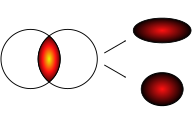
\includegraphics[width=\textwidth]{ellipticflow_viscous}};
      \node[anchor=north,xshift=2.5ex,text width=10ex,text centered] at (fig.north) {small $\eta/s$ \\ large $v_2$};
      \node[anchor=south,xshift=2.5ex,text width=10ex,text centered] at (fig.south) {large $\eta/s$ \\ small $v_2$};
    \end{tikzpicture}

    \column{.55\textwidth}
    \begin{itemize}
      \item Observe experimental $v_n$.
      \item Run model with variable $\eta/s$.
      \item Constrain $\eta/s$ by matching $v_n$.
    \end{itemize}
  \end{columns}

  \bgs
  \centering
  \includegraphics[width=.8\textwidth]{osu2} \\
  \flushright\tiny
  H.~Song, S.~A.~Bass, U.~Heinz, T.~Hirano and C.~Shen,
  PRL\ {\bf 106}, 192301 (2011).

\end{frame}




\begin{frame}{Extracting QGP properties}
  \begin{columns}
    \column{.50\textwidth}
    %\hfill\tikz[overlay,remember picture] \node (top) {};
    \begin{itemize}
      \item Average flow $\avg{v_n}$.
      \item Vary only $\eta/s$, other parameters fixed.
      \item Only several discrete values.
      \item Qualitative constraints lacking uncertainty.
    \end{itemize}
    %\hfill\tikz[overlay,remember picture] \node (bottom) {};
    %\tikz[overlay,remember picture] \draw [decorate,decoration={brace,amplitude=0.5em},thick] (top) -- (bottom);

    %\column{.03\textwidth}
    %$\large\boldsymbol\Longrightarrow$

    \column{.50\textwidth}
    \begin{itemize}
      \item Event-by-event flow $P(v_n)$.
      \item Vary all salient parameters:  $\eta/s$, $\tau_0$, IC parameters, \ldots
      \item Continuous parameter space.
      \item Quantitative constraints including uncertainty.
    \end{itemize}
  \end{columns}

  \tikz[overlay,remember picture] \node[yshift=2ex] at (current page.center) {$\large\boldsymbol\Longrightarrow$};
\end{frame}



\section{Method}



\begin{frame}{Computer experiments with slow models}
  \begin{columns}[t]
    \column{.5\textwidth}
    %\begin{center}
    %  \bf Challenges
    %\end{center}
    %\vspace{-2.2pt}
    %\hrule
    %\strut Challenges
    \begin{center}
      \large\bf
      \strut Challenges
    \end{center}
    \begin{itemize}
      \item Event-by-event models very computationally expensive, ${\sim}1$ hour per event.
      \item Need $\mathcal O(10^3)$ events per parameter-point to study fluctuations.
      \item Must vary all parameters simultaneously.
    \end{itemize}

    \column{.5\textwidth}
    %\textbf{Solutions}
    %\begin{center}
    %  \bf Solutions
    %\end{center}
    %\hrule
    \begin{center}
      \large\bf
      \strut Strategies
    \end{center}
    \begin{itemize}
      \item Evaluate model at efficient pre-determined parameter points.
        \begin{itemize}
          \item Latin-hypercube sampling.
        \end{itemize}
      \item Interpolate between explicitly calculated points.
        \begin{itemize}
          \item Gaussian process emulator.
        \end{itemize}
    \end{itemize}
  \end{columns}
\end{frame}


\begin{frame}{Latin-hypercube sampling}
  \begin{itemize}
    \item Random set of parameter points.
    \item Maximizes CPU time efficiency.
    \item Skeleton of parameter space.
  \end{itemize}

  \bgs 

  \centering
  %\tikz\draw[thick] (0,0) rectangle node {LHS samples} (\textwidth,.35\textwidth);
  \includegraphics{lhs}
  %\includegraphics<2>{lhs2}
\end{frame}


\begin{frame}[label=gp]{Gaussian processes}

  %A Gaussian \emph{process} is a generalization of a Gaussian \emph{distribution}:  \\
  %instead of drawing random numbers, draw random functions. {\color{red} formal definition} \\[1.5em]

  \begin{itemize}
    %\item A Gaussian process is a stochastic process where each point is normally distributed.
    \item \emph{A Gaussian process is a collection of random variables, any finite number of which have a joint Gaussian distribution.}
    \item Instead of drawing variables from a distribution, functions are drawn from a process.
  \end{itemize}



  \begin{columns}[c]
    \column{.55\textwidth}
    Require a covariance function, e.g.
    \begin{equation*}
      \text{cov}(x_1,x_2) \propto \exp \biggl[ -\frac{(x_1 - x_2)^2}{2\ell^2} \biggr]
    \end{equation*}
    Nearby points correlated, distant points independent.

    \column{.45\textwidth}
    \hyperlink{gengp}{\includegraphics[width=\textwidth]{gpr1}} \\[1ex]
    \raggedleft\tiny \emph{Gaussian Processes for Machine Learning}, \\ Rasmussen and Williams, 2006.
  \end{columns}

\end{frame}


\begin{frame}[label=emu]{Gaussian process emulators}
  \begin{itemize}
    \item Prior:  the model is a Gaussian process.
    \item Posterior:  Gaussian process conditioned on model outputs.
  \end{itemize}

  %\sms

  \hspace{-5mm}
  \begin{tikzpicture}
    \draw[thick,->] (0,0) node[left] (prior) {\includegraphics[width=.41\textwidth]{gpr1}} -- 
    node[above] {\hyperlink{training}{Training}} (1.8,0) node[right] (posterior) {\includegraphics[width=.41\textwidth]{gpr2}};
    \node[xshift=1.2ex] at (prior.north) {Prior};
    \node[xshift=1.5ex] at (posterior.north) {Posterior};
    %\node[align=right,anchor=east] at (posterior.south east) {\tiny Rasmussen and Williams, \emph{Gaussian processes for machine learning}.};
  \end{tikzpicture}
  
  %\sms

  \begin{itemize}
    \item Emulator is a fast surrogate to the actual model.
      \begin{itemize}
        \item More certain near calculated points.
        \item Less certain in gaps.
      \end{itemize}
  \end{itemize}
\end{frame}




\begin{frame}[label=atlas]{Experimental data}
  \begin{itemize}
    \item ATLAS event-by-event flow distributions $v_2,v_3,v_4$.
    \item Fit to \hyperlink{rice}{Rice / Bessel-Gaussian distribution}
      \begin{equation*}
        P(v_n) = \frac{v_n}{\delta_{v_n}^2} e^{ -\frac{(v_n)^2 + (v_n^\text{RP})^2}{2\delta_{v_n}^2} }
        I_0 \pfrac{v_n^\text{RP}v_n}{\delta_{v_n}^2}
      \end{equation*}
    \item Reduce to parameters $v_n^\text{RP}$, $\delta_{v_n}$.
  \end{itemize}
  
  %\vspace{-3ex}


  \centering
  \hyperlink{unfold}{\includegraphics[width=\textwidth]{atlas}}
  \flushright\vspace{-2ex} \tiny ATLAS Collaboration, JHEP {\bf 1311}, 183 (2013).
\end{frame}



\begin{frame}{Event-by-event model}
  Modern version of Duke+OSU model VISHNU \mbox{(Viscous Hydro and UrQMD)}:
  \begin{itemize}
    \item MC-Glauber \& MC-KLN initial conditions \\
      \hspace{1em} {\tiny H.-J.\ Drescher and Y.\ Nara, Phys.\ Rev.\ C {\bf 74}, 044905 (2006).}
    \item Viscous hydro \\
      \hspace{1em} {\tiny H.\ Song and U.\ Heinz, Phys.\ Rev.\ C {\bf 77}, 064901 (2008).}
    \item Cooper-Frye sampler \\
      \hspace{1em} {\tiny Z.\ Qiu and C.\ Shen, arXiv:1308.2182 [nucl-th].}
    \item UrQMD (Ultrarelativistic Quantum Molecular Dynamics) \\
      \hspace{1em} {\tiny S.\ Bass \emph{et.\ al.}, Prog.\ Part.\ Nucl.\ Phys.\  {\bf 41}, 255 (1998).} \\[-1ex]
      \hspace{1em} {\tiny M.\ Bleicher \emph{et.\ al.}, J.\ Phys.\ G {\bf 25}, 1859 (1999).}
  \end{itemize}

  \mds
  $\color{theme}\boldsymbol\rarr$ Tailored for running many events on Open Science Grid.
  
  %\vspace{.07\textheight}

  %\centering
  %\begin{tabular}{ll}
  %  \toprule
  %  Input parameters & Observables \\
  %  \midrule
  %  Normalization                           & \\
  %  WN/BC $\alpha$                          & $v_n$ distributions \\
  %  Thermalization time $\tau_0$            & Multiplicities \\
  %  Viscosity $\eta/s$                      & \ldots \\
  %  Shear relaxation time $\tau_\Pi$ & \\
  %  \bottomrule
  %\end{tabular}

\end{frame}





\begin{frame}{Computer experiment design}
  \begin{itemize}
    \item Six centrality bins 0--5\%, 10--15\%, \ldots\ 50--55\%.
    \item 256 Latin-hypercube points, five input parameters:
      \begin{itemize}
        \item Normalization
        \item IC-specific parameter
        \item Thermalization time $\tau_0$
        \item Viscosity $\eta/s$
        \item Shear relaxation time $\tau_\Pi$
      \end{itemize}
  \end{itemize}
  \begin{itemize}
    \item Massive parallelization on Open Science Grid.
    \item Completed 1000--2000 events per centrality bin and input-parameter point.
      \begin{itemize}
        \item 3.5 million total
        \item 0.5 $\mu\text{b}^{-1}$  (ATLAS:  7 $\mu\text{b}^{-1}$)
      \end{itemize}
  \end{itemize}

  %\bgs
  %\begin{itemize}
  %  \item (6 centrality bins) $\times$ (3 flow coefficients) = 18 flow ``categories''
  %  \item $v_2$ 0--5\% and $v_2$ 40--45\% are representative.
  %\end{itemize}
\end{frame}


\begin{frame}{Open Science Grid usage}
  \begin{tikzpicture}
    \node (fig) {\includegraphics[width=\textwidth]{osghours}};
    \node[anchor=south,yshift=-1ex,xshift=1.7ex] at (fig.north) {CPU hours per day};
    \node[anchor=south west,yshift=-1ex,xshift=1ex] at (fig.north west) {\small 250,000};
    \node[anchor=south west,yshift=1.8cm,xshift=.8cm] at (fig) {red = Me};
  \end{tikzpicture}
  \centering
  Completed KLN design (1.5 million events) in two weeks.
\end{frame}


\againframe{mtd}


\section{Results}


\begin{frame}{Model flow distributions}
  \vspace{6mm}
  \hspace{-3mm}
  \includegraphics{allcurves}
  %\the\textheight
  %\tikz\draw (0,0) rectangle (\textwidth,.8\textheight);
\end{frame}



\begin{frame}[label=scatter]{Input-output summary}
  \vspace{6mm}
  \hspace{-3mm}
  \hyperlink{linear}{
    \includegraphics<1>{scatters-glb}
    \includegraphics<2>{scatters-kln}
  }
\end{frame}




\begin{frame}{Best parameter points}
  \begin{columns}
    \column{.6\textwidth}
    \vspace{3mm}

    \scriptsize\raggedleft Best Latin-hypercube points by average $v_n$\ \ \ \\[.5ex]
    \includegraphics{bestavg}

    \column{.4\textwidth}
    %\begin{tabular}{lllll}
    %  \toprule
    %  & $\alpha\mid\lambda$ & $\tau_0$ & $\eta/s$
    %  \midrule
    %  \bottomrule
    %\end{tabular}
    %\begin{equation*}
    %  \alpha = 0.27,\;
    %  \tau_0 = 0.46 \ut{fm/c},\;
    %  \eta/s = 0.026,\;
    %  \tau_\Pi = 1.0 \ut{fm/c};
    %\end{equation*}
    %\begin{equation*}
    %  \lambda = 0.25,\;
    %  \tau_0 = 0.70 \ut{fm/c},\;
    %  \eta/s = 0.21,\;
    %  \tau_\Pi = 0.28 \ut{fm/c}.
    %\end{equation*}
    \small
    OSU results, same model \\[1em]
    dashed: Glauber $\eta/s = 0.08$ \\
    solid: KLN $\eta/s = 0.20$ \\[1ex]
    \begin{tikzpicture}
      \small
      \node (fig) {\includegraphics[width=\textwidth]{osu}};
      \node[anchor=east,shift=({-1.2em,3.2em})] at (fig.east) {$v_2$};
      \node[anchor=east,shift=({-1.2em,-1.3em})] at (fig.east) {$v_3$};
    \end{tikzpicture} \\
    %\includegraphics[width=\textwidth]{osu} \\
    \raggedleft\tiny Z. Qiu, C. Shen, and U.~Heinz, \\ Phys.\ Lett.\ B {\bf 707}, 151 (2012).
  \end{columns}
\end{frame}



\begin{frame}{Constraining $\eta/s$}
  \vspace{3mm}
  \small
  Points:  average $\eta/s$ of best 10 Latin-hypercube points by average $v_n$ \\
  Error bars:  standard deviation of best 10 \\
  Dashed lines:  canonical $\eta/s$ (Glauber 0.08, KLN 0.20) \\[1em]
  \includegraphics{preferredeta}
\end{frame}



\begin{frame}{Bessel-Gaussian parameters (Glauber)}
  \vspace{3mm}
  \includegraphics{bgparams}
\end{frame}


\begin{frame}[label=emuplots]{Emulated Bessel-Gaussian parameters}
  \vspace{3mm}
  \hyperlink{caveats}{
    \includegraphics<1>{emu0}
    \includegraphics<2>{emu1}
    \includegraphics<3>{emu2}
  }
\end{frame}


\section{Conclusion}

\begin{frame}[label=conc]{Summary \& outlook}
  \begin{itemize}
    \item Framework for massive event-by-event model-to-data comparison:  new level of knowledge-extraction capability.
    \item Preliminary results consistent with previous work.
      \bgs
    \item Improve flow distribution parameter estimates.
    \item Validate emulator.
    \item Calculate posterior distributions \\
      $\rarr$ extract optimal values of parameters with uncertainty.
    \item Calibrate simultaneously on other observables, e.g.\ multiplicity.
    \item Repeat with more advanced models, especially initial conditions.
  \end{itemize}
\end{frame}



\appendix

\def\backbutton#1{
  \tikz[remember picture,overlay]\node[anchor=south west] at (current page.south west) {\hyperlink{#1}{\footnotesize\color{theme}$\blacktriangleleft$}};
}

\begin{frame}[plain,noframenumbering]{}
  \centering
  \Large
  backup slides
\end{frame}


\begin{frame}[label=gengp]{Generating Gaussian processes}
  \begin{columns}
    \column{.67\textwidth}
    \begin{itemize}
      \item Choose a set of input points $X_*$.
      \item Choose a covariance function, e.g.\
        \begin{equation*}
          k(x_i,x_j) = \exp[-(x_i-x_j)^2/2]
        \end{equation*}
        and create covariance matrix $K(X_*,X_*)$.
      \item Generate MVN samples (GPs)
        \begin{equation*}
          \vec f_* \sim \mathcal N[\vec 0,K(X_*,X_*)].
        \end{equation*}
    \end{itemize}

    \column{.33\textwidth}
    \includegraphics[width=\textwidth]{gpr1}
  \end{columns}

  \backbutton{gp}
\end{frame}


\begin{frame}[label=training]{Training the emulator}
  \begin{itemize}
    \item Make observations $\vec f$ at training points $X$.
    \item Generate conditioned GPs
        \begin{align*}
          \vec f_* | X_*,X,\vec f &\sim \mathcal N[K(X_*,X)K(X,X)^{-1}\vec f, \\
          &\qquad {} K(X_*,X_*) - K(X_*,X)K(X,X)^{-1}K(X,X_*)].
        \end{align*}
  \end{itemize}

  \centering

  \begin{tikzpicture}
    \draw[thick,->] (0,0) node[left] (prior) {\includegraphics[width=.35\textwidth]{gpr1}} -- (1,0) node[right] (posterior) {\includegraphics[width=.35\textwidth]{gpr2}};
    \node[xshift=1.2ex] at (prior.north) {Prior};
    \node[xshift=1.5ex] at (posterior.north) {Posterior};
  \end{tikzpicture}

  \backbutton{emu}
\end{frame}


\begin{frame}[label=rice]{Rice / Bessel-Gaussian distribution}
  \vspace{1em}

  \begin{itemize}
    \item Flow vectors follow bivariate Gaussian
      \begin{equation*}
        P(\vec v_n) = \frac{1}{2\pi\delta_{v_n}^2} e^{ -\frac{(\vec v_n - \vec v_n^\text{RP})^2}{2\delta_{v_n}^2} }.
      \end{equation*}
    \item Integrate out angle
      \begin{equation*}
        P(v_n) = \frac{v_n}{\delta_{v_n}^2} e^{ -\frac{(v_n)^2 + (v_n^\text{RP})^2}{2\delta_{v_n}^2} }
          I_0 \pfrac{v_n^\text{RP}v_n}{\delta_{v_n}^2}.
      \end{equation*}
  \end{itemize}

  \vspace{1em}

  \centering
  \includegraphics[width=.7\textwidth]{rice}
  
  \backbutton{atlas}
\end{frame}


\begin{frame}[label=unfold]{Finite multiplicity and unfolding}
  \def\obs{^\text{obs}}

  \begin{itemize}
    \item Observed flow smeared by finite multiplicity and nonflow
      \begin{equation*}
        P(v_n\obs) = \int P(v_n\obs|v_n) P(v_n) \, dv_n
      \end{equation*}
      where $P(v_n\obs|v_n)$ is the response function.
    \item Pure statistical smearing $\rarr$ Gaussian response
      \begin{equation*}
        P(v_n^\text{obs}|v_n) = \frac{v_n^\text{obs}}{\delta_{v_n}^2} e^{ -\frac{(v_n^\text{obs})^2 + (v_n)^2}{2\delta_{v_n}^2} }
          I_0 \pfrac{v_nv_n^\text{obs}}{\delta_{v_n}^2}.
      \end{equation*}
    \item $v_n^\text{RP}$ unaffected; width increased as
      \begin{equation*}
        \delta_{v_n}^2 \rarr \delta_{v_n}^2 + 1/2M.
      \end{equation*}
  \end{itemize}

  \backbutton{atlas}
\end{frame}


\begin{frame}[label=caveats]{Caveats}
  \begin{itemize}
    \item Results still qualitative.
    \item Some Bessel-Gaussian fit parameters are incorrect (MLE two-solution problem / low SNR).
    \item Uncertainties not quantified.
    \item Parameter space not systematically explored.
  \end{itemize}

  \backbutton{emuplots}
\end{frame}






\end{document}
